\documentclass[11pt]{article}
\usepackage{worksheet_style}

% ---- Toggle: uncomment for filled version ----
%\worksheetfilledtrue
\begin{document}
\worksheetheader{2}{Vectors in $\R^3$}

\begin{background}
Last time we set up 3D coordinates. Now we need a language to describe direction and magnitude in space---that's what vectors give us. Vectors are the building blocks of everything in this course: lines, planes, curves, derivatives, integrals, and fields all use vector notation.
\end{background}

%=============================================================
\wsection{Vectors --- Definitions}

\begin{defbox}{Vector}
A \textbf{vector} is a quantity carrying both \wbi{magnitude}{2cm} and \wbi{direction}{2cm} — visually, an arrow. Two arrows are considered the \emph{same} vector whenever they have the same length and direction, no matter where they are drawn, so a vector is really an equivalence class of parallel arrows. Placing its tail at the origin, the tip lands at a specific point $(v_1,v_2,v_3)$, and those coordinates are the \textbf{components} of $\vect{v}$.

\medskip
-- Written $\vect{v} = \vec{v_1, v_2, v_3}$; angle brackets distinguish vectors from points $(a,b,c)$
\end{defbox}

\begin{center}
\tdplotsetmaincoords{65}{140}
\begin{tikzpicture}[scale=3.8, tdplot_main_coords]
\pgfmathsetmacro{\vx}{0.6}
\pgfmathsetmacro{\vy}{0.5}
\pgfmathsetmacro{\vz}{0.7}
\draw[->, thick] (0,0,0) -- (1.2,0,0) node[anchor=west] {$x$-axis};
\draw[->, thick] (0,0,0) -- (0,1.2,0) node[anchor=west] {$y$-axis};
\draw[->, thick] (0,0,0) -- (0,0,1.2) node[anchor=south] {$z$-axis};
\draw[->, blue!70!black, ultra thick] (0,0,0) -- (\vx,\vy,\vz) node[anchor=south] {$(x, y, z)$};
\draw[dashed, blue!50] (\vx, \vy, \vz) -- (\vx, \vy, 0);
\draw[dashed, blue!50] (\vx, \vy, \vz) -- (\vx, 0, \vz);
\draw[dashed, blue!50] (\vx, \vy, \vz) -- (0, \vy, \vz);
\filldraw[blue!50] (\vx, \vy, 0) circle (0.4pt);
\filldraw[blue!50] (\vx, 0, \vz) circle (0.4pt);
\filldraw[blue!50] (0, \vy, \vz) circle (0.4pt);
\end{tikzpicture}\\
{\small A vector in $\R^3$ represented by its components along the $x$, $y$, and $z$ axes. Dashed lines mark the projections onto the three coordinate planes.}
\end{center}

\begin{defbox}{Magnitude (Norm)}
The \textbf{magnitude} (or \textbf{norm}) $\|\vect{v}\|$ is the length of the vector — the Euclidean distance from its tail to its tip. When $\vect{v}$ is drawn with its tail at the origin, $\|\vect{v}\|$ is literally the distance from the origin to the terminal point, and it is unchanged by rotating or translating the coordinate system. In short, magnitude strips away direction and records only \emph{how much} of the vector there is. It is computed by the Pythagorean theorem applied to the components:
\[\|\vect{v}\| = \wbml{\sqrt{v_1^2 + v_2^2 + v_3^2}}\]
\end{defbox}

\begin{defbox}{Unit Vector}
A vector with magnitude \wbi{1}{1cm}. To \textbf{normalize}:
\[\uvec{v} = \wbml{\frac{\vect{v}}{\|\vect{v}\|}}\]
Standard unit vectors: $\ihat = \vec{1,0,0}$, \; $\jhat = \vec{0,1,0}$, \; $\khat = \vec{0,0,1}$
\end{defbox}

\begin{defbox}{Direction Cosines}
For $\vect{v} = \vec{a,b,c}$, the angles $\alpha, \beta, \gamma$ with the $x$-, $y$-, $z$-axes:
\[\cos\alpha = \wbm{\frac{a}{\|\vect{v}\|}}, \quad \cos\beta = \wbm{\frac{b}{\|\vect{v}\|}}, \quad \cos\gamma = \wbm{\frac{c}{\|\vect{v}\|}}\]
Key identity: $\cos^2\alpha + \cos^2\beta + \cos^2\gamma = \wbm{1}$
\end{defbox}

\begin{formulabox}{Vector Arithmetic}
If $\vect{u} = \vec{u_1, u_2, u_3}$ and $\vect{v} = \vec{v_1, v_2, v_3}$:
\begin{align*}
  \vect{u} + \vect{v} &= \wbml{\vec{u_1+v_1,\; u_2+v_2,\; u_3+v_3}} \\
  c\,\vect{u} &= \wbml{\vec{cu_1,\; cu_2,\; cu_3}}
\end{align*}
-- Addition is ``tip-to-tail''; scalar multiplication scales length
\end{formulabox}

\begin{center}
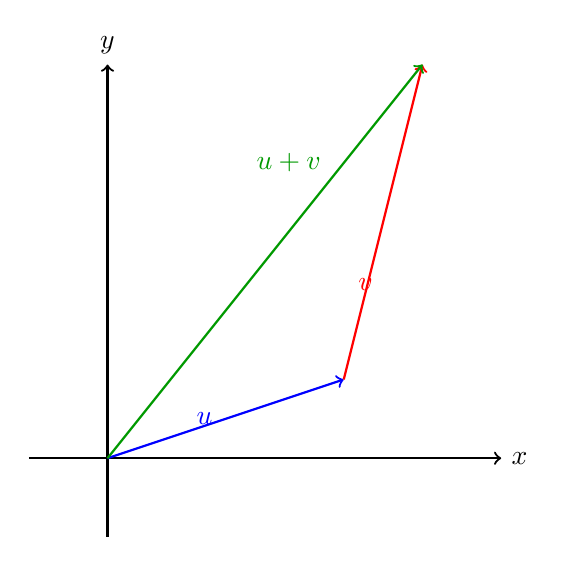
\begin{tikzpicture}
\draw[thick,->] (-1,0) -- (5,0) node[right] {$x$};
\draw[thick,->] (0,-1) -- (0,5) node[above] {$y$};
\draw[thick,->,blue] (0,0) -- (3,1) node[anchor=south west] at (1,0.3) {$\vect{u}$};
\draw[thick,->,red] (3,1) -- (4,5) node[anchor=south east] at (3.5,2) {$\vect{v}$};
\draw[thick,->,green!60!black] (0,0) -- (4,5) node[anchor=south] at (2.3,3.5) {$\vect{u} + \vect{v}$};
\end{tikzpicture}\\
{\small Tip-to-tail method of vector addition: placing $\vect{v}$ at the tip of $\vect{u}$ results in $\vect{u}+\vect{v}$.}
\end{center}

%=============================================================
\wsection{The Dot Product}

\begin{defbox}{Dot Product}
\textbf{Component formula:}
\[\vect{u}\cdot\vect{v} = \wbml{u_1 v_1 + u_2 v_2 + u_3 v_3}\]

\textbf{Geometric formula:}
\[\vect{u}\cdot\vect{v} = \wbml{\|\vect{u}\|\,\|\vect{v}\|\cos\theta}\]
-- The dot product is a \wbi{scalar}{1.5cm} (number, not a vector)
\end{defbox}

\begin{formulabox}{Dot Product Facts}
\begin{itemize}[nosep, leftmargin=*]
  \item $\vect{u} \perp \vect{v}$ $\iff$ $\vect{u}\cdot\vect{v} = \wbm{0}$
  \item Angle between vectors: $\theta = \wbm{\arccos\!\left(\dfrac{\vect{u}\cdot\vect{v}}{\|\vect{u}\|\,\|\vect{v}\|}\right)}$
\end{itemize}
\end{formulabox}

\begin{defbox}{Vector Projection}
The \textbf{projection} of $\vect{u}$ onto $\vect{v}$ is the ``shadow'' that $\vect{u}$ casts along the line of $\vect{v}$ — the part of $\vect{u}$ that points in the direction of $\vect{v}$. It is a vector parallel to $\vect{v}$ whose length is the \emph{scalar component} $\comp_{\vect{v}}\vect{u}=\|\vect{u}\|\cos\theta$.
\[\proj_{\vect{v}} \vect{u} = \wbml{\frac{\vect{u}\cdot\vect{v}}{\|\vect{v}\|^2}\,\vect{v}}\]

Scalar component:
\[\comp_{\vect{v}} \vect{u} = \wbml{\frac{\vect{u}\cdot\vect{v}}{\|\vect{v}\|}}\]
\end{defbox}

\begin{center}
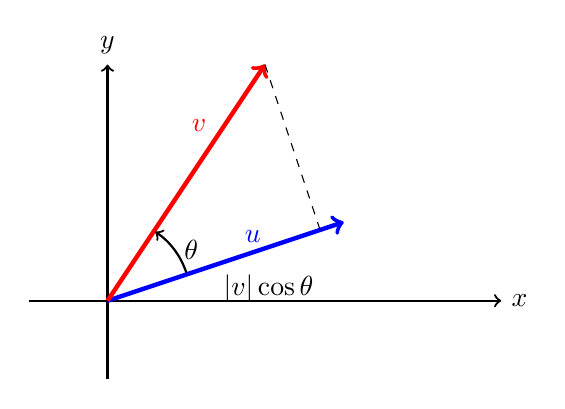
\begin{tikzpicture}
\draw[thick,->] (-1,0) -- (5,0) node[right] {$x$};
\draw[thick,->] (0,-1) -- (0,3) node[above] {$y$};
\draw[ultra thick,->,blue] (0,0) -- (3,1) node[anchor=south west] at (1.6,0.6) {$\vect{u}$};
\draw[ultra thick,->,red] (0,0) -- (2,3) node[anchor=south east] at (1.4,2) {$\vect{v}$};
\draw[dashed] (2,3) -- (2.7,0.9);
\draw[thick,->] (1,.36) arc[start angle=18.4,end angle=56.3,radius=1] node[midway, right] {$\theta$};
\node[anchor=north west] at (1.35,0.45) {$|\vect{v}| \cos \theta$};
\end{tikzpicture}\\
{\small The dot product interpreted as the projection of $\vect{v}$ onto $\vect{u}$, scaled by $\cos\theta$.}
\end{center}

\begin{example}[Crane Cable Forces]
Two crane cables exert forces $\vect{F}_1 = \vec{120, 0, 80}$ N and $\vect{F}_2 = \vec{-50, 75, 60}$ N.
\begin{enumerate}[label=(\alph*), nosep]
  \item Find the total force $\vect{F}_1 + \vect{F}_2$.
  \item Find a unit vector in the direction of the total force.
  \item What force $\vect{F}_3$ would perfectly counterbalance $\vect{F}_1 + \vect{F}_2$?
\end{enumerate}

\wbbox{
1. Total force:
\[\vect{F}_1 + \vect{F}_2 = \vec{70, 75, 140} \text{ N}\]

2. Magnitude:
\[\|\vect{F}_1+\vect{F}_2\| = \sqrt{70^2+75^2+140^2} = \sqrt{4900+5625+19600} = \sqrt{30125} \approx 173.6 \text{ N}\]

3. Unit vector:
\[\uvec{F} = \frac{1}{173.6}\vec{70, 75, 140} \approx \vec{0.403, 0.432, 0.807}\]

4. Counterbalance: $\vect{F}_3 = -(\vect{F}_1 + \vect{F}_2) = \vec{-70, -75, -140}$ N
}{5cm}
\end{example}

\begin{example}[Dot Product and Angle]
Let $\vect{a} = \vec{3, 0, 4}$ and $\vect{b} = \vec{1, 2, -1}$. Find $\vect{a}\cdot\vect{b}$ and the angle between them.

\wbbox{
1. Dot product:
\[\vect{a}\cdot\vect{b} = (3)(1)+(0)(2)+(4)(-1) = 3+0-4 = -1\]

2. Magnitudes:
\[\|\vect{a}\| = \sqrt{9+0+16} = 5, \qquad \|\vect{b}\| = \sqrt{1+4+1} = \sqrt{6}\]

3. Angle:
\[\cos\theta = \frac{-1}{5\sqrt{6}} \quad\implies\quad \theta = \arccos\!\left(\frac{-1}{5\sqrt{6}}\right) \approx 94.7^\circ\]

Since $\theta > 90^\circ$, the vectors point in ``generally opposite'' directions.
}{4cm}
\end{example}

\begin{example}[Projection]
Project $\vect{a} = \vec{3,4,5}$ onto $\vect{n} = \vec{1,1,1}$.

\wbbox{
1. Compute pieces:
\[\vect{a}\cdot\vect{n} = 3+4+5 = 12, \qquad \|\vect{n}\|^2 = 3\]

2. Projection:
\[\proj_{\vect{n}}\vect{a} = \frac{12}{3}\vec{1,1,1} = \vec{4,4,4}\]

3. Perpendicular component: $\vect{a} - \proj_{\vect{n}}\vect{a} = \vec{3,4,5} - \vec{4,4,4} = \vec{-1, 0, 1}$
}{3.5cm}
\end{example}

%=============================================================
\wsection{The Cross Product}

\begin{defbox}{Cross Product}
\textbf{Determinant formula:}
\[\vect{u}\times\vect{v} = \wbml{\begin{vmatrix} \ihat & \jhat & \khat \\ u_1 & u_2 & u_3 \\ v_1 & v_2 & v_3 \end{vmatrix} = \vec{u_2 v_3 - u_3 v_2,\; u_3 v_1 - u_1 v_3,\; u_1 v_2 - u_2 v_1}}\]

\textbf{Properties:}
\begin{itemize}[nosep]
  \item $\vect{u}\times\vect{v}$ is \wbi{perpendicular to both $\vect{u}$ and $\vect{v}$}{6cm}
  \item $\|\vect{u}\times\vect{v}\| = \wbm{\|\vect{u}\|\,\|\vect{v}\|\sin\theta}$ -- area of parallelogram
  \item Direction via the \wbi{right-hand rule}{3cm}
  \item $\vect{u}\times\vect{v} = \wbm{-\vect{v}\times\vect{u}}$ (anti-commutative)
\end{itemize}
\end{defbox}

\begin{center}
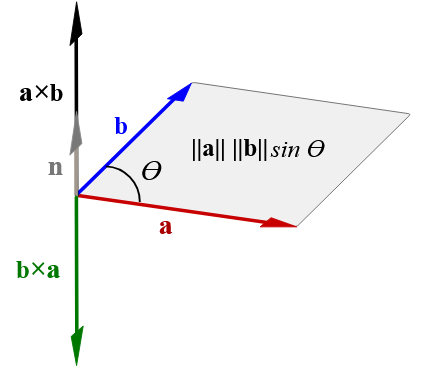
\includegraphics[width=6cm]{pics/cross_prod.png}\\
{\small Cross product: $\vect{a}\times\vect{b}$ is perpendicular to both, with magnitude $= \|\vect{a}\|\|\vect{b}\|\sin\theta$ (parallelogram area).}
\end{center}

\begin{formulabox}{Cross Product Facts}
\begin{itemize}[nosep, leftmargin=*]
  \item $\vect{u} \parallel \vect{v} \iff \vect{u}\times\vect{v} = \wbm{\vect{0}}$
  \item $\ihat\times\jhat = \khat$, \; $\jhat\times\khat = \ihat$, \; $\khat\times\ihat = \jhat$
  \item $\vect{u}\times\vect{u} = \vect{0}$ always
\end{itemize}
\end{formulabox}

\begin{example}[Cross Product Computation]
Compute $\vect{a}\times\vect{b}$ for $\vect{a} = \vec{3,0,4}$ and $\vect{b} = \vec{1,2,-1}$.

\wbbox{
1. Set up the determinant:
\[\vect{a}\times\vect{b} = \begin{vmatrix} \ihat & \jhat & \khat \\ 3 & 0 & 4 \\ 1 & 2 & -1\end{vmatrix}\]

2. Expand:
\[= \ihat(0\cdot(-1) - 4\cdot 2) - \jhat(3\cdot(-1) - 4\cdot 1) + \khat(3\cdot 2 - 0\cdot 1) = \vec{-8, 7, 6}\]

3. Verify orthogonality: $\vect{a}\cdot(\vect{a}\times\vect{b}) = (3)(-8)+(0)(7)+(4)(6) = -24+0+24 = 0$ \;\checkmark
}{4cm}
\end{example}

%=============================================================
\wsection{Scalar Triple Product}

\begin{formulabox}{Scalar Triple Product}
$\vect{a}\cdot(\vect{b}\times\vect{c})$ -- gives the \wbi{volume of the parallelepiped}{4cm} spanned by $\vect{a}, \vect{b}, \vect{c}$

\[\text{Volume} = |\vect{a}\cdot(\vect{b}\times\vect{c})|\]
\end{formulabox}

\begin{example}[Scalar Triple Product --- Volume]
Find the volume of the parallelepiped spanned by $\vect{a} = \vec{1,0,2}$, $\vect{b}=\vec{3,1,0}$, $\vect{c}=\vec{0,2,1}$.

\wbbox{
1. Cross product $\vect{b}\times\vect{c}$:
\[\vect{b}\times\vect{c} = \begin{vmatrix} \ihat & \jhat & \khat \\ 3 & 1 & 0 \\ 0 & 2 & 1\end{vmatrix} = \vec{1, -3, 6}\]

2. Triple product:
\[\vect{a}\cdot(\vect{b}\times\vect{c}) = (1)(1)+(0)(-3)+(2)(6) = 13\]

3. Result: Volume $= |13| = \boxed{13}$ cubic units.
}{4cm}
\end{example}

%=============================================================
\vspace{6pt}
\textit{Show all work for full credit.}

\begin{practice}

\prob Let $\vect{v} = \vec{3, 4, 12}$. Find $\|\vect{v}\|$, the unit vector $\uvec{v}$, and the direction cosines.

\wans{$\|\vect{v}\| = \wbm{13}$, \; $\uvec{v} = \wbml{\vec{3/13,\; 4/13,\; 12/13}}$

Direction cosines: $\cos\alpha = \wbm{3/13}$, $\cos\beta = \wbm{4/13}$, $\cos\gamma = \wbm{12/13}$}

\vspace{2cm}

\prob Compute $\vect{u}\cdot\vect{v}$ and $\vect{u}\times\vect{v}$ for $\vect{u} = \vec{2, -1, 3}$ and $\vect{v} = \vec{4, 0, -2}$.

\wans{$\vect{u}\cdot\vect{v} = \wbm{2}$, \quad $\vect{u}\times\vect{v} = \wbml{\vec{2, 16, 4}}$}

\vspace{2.5cm}

\prob Find the angle between $\vect{u} = \vec{1, 1, 0}$ and $\vect{v} = \vec{0, 1, 1}$.

\wans{$\theta = \wbm{\pi/3 = 60^\circ}$}

\vspace{2.5cm}

\prob Find $\proj_{\vect{n}}\vect{a}$ where $\vect{a} = \vec{3,4,5}$ and $\vect{n} = \vec{1,1,1}$. Also find the perpendicular component.

\wans{$\proj_{\vect{n}}\vect{a} = \wbml{\vec{4,4,4}}$, \quad perpendicular component $= \wbml{\vec{-1, 0, 1}}$}

\vspace{2.5cm}

\prob Three points $P_1=(1,2,3)$, $P_2=(4,-1,2)$, $P_3=(-2,3,5)$ define a plane. Use the cross product to find a normal vector.

\wans{$\vect{n} = \wbml{\vec{-5, -3, -6}}$}

\vspace{3cm}

\prob Find the volume of the parallelepiped spanned by $\vect{a} = \vec{2,1,0}$, $\vect{b} = \vec{1,-1,3}$, $\vect{c} = \vec{0,2,1}$.

\wans{Volume $= \wbm{13}$}

\vspace{2.5cm}

\end{practice}

\end{document}
